\apendice{Especificación de diseño}

\section{Introducción}
Este tercer apéndice tratará el diseño de los datos usados en la aplicación, junto con el diseño procedimental y el diseño arquitectónico.

\section{Diseño de datos}
En este subpunnto se recogen la información relevante de las tres tablas de datos que nos ha dado la empresa para poder realizar el proyecto. Además, se explican los diferentes sensores que hay, junto con su identificación para su posible comprensión. Esta descripción es muy importante, porque son los datos con los que se ha podido llevar a cabo el proyecto, y es importante que cualquier persona los pueda comprender para entender claramente que se ha efectuado en el código desarrollado.

A continuación se recoge el nombre de cada tabla junto con los atributos más relevantes (aquellos que han sido utilizados a lo largo del proyecto):

\begin{itemize}
    \item \textbf{Gauges:} contiene un total de 6 valores, que se corresponden con los diferentes sensores de la empresa. A continuación, se muestra la ID de cada sensor junto con sus principales características:
        \begin{itemize}
        \item \textbf{123:} se corresponde con un sensor de datos 1D que mide la capa superior de la bobina. Toma datos cada 10 metros.
        \item \textbf{124:} se corresponde con la pareja del sensor 123, pero toma datos de la capa inferior de la bobina.
        \item \textbf{201:} se corresponde con otro sensor de datos 1D, pero diferente al anteriomente mencionado, de la capa superior.
        \item \textbf{202:} es la pareja del sensor 201. Toma medida de la capa inferior de la bobina.
        \item \textbf{1234:} es un sensor de los datos 2D y toma datos de la capa superior de la bobina.
        \item \textbf{1243:} es la pareja del sensor 1234, y toma datos de la capa inferior de la bobina.
        \end{itemize}
    \item \textbf{GR\_LPValues:} contiene los registros de los datos 1D. Cada registro se corresponde para una bobina, sensor y teja específica. Los principales atributos son:
    \begin{itemize}
        \item \textbf{COILID:} se corresponde con la ID de la bobina.
        \item \textbf{TILEID:} se corresponde con la ID de la teja de la bobina. Cada teja tiene diferentes ID, su orden es cronológico, es decir, la prima teja será el valor más pequeño, la segunda teja, el segundo valor más pequeño, y así sucesivamente.
        \item \textbf{MID:} se corresponde con la ID del sensor que ha capturado los datos. Estos valores son los mencionados anteriormente en la tabla \emph{Gauges}.
        \item \textbf{MEAN:} contiene el valor medio de zinc en dicha teja. Este es el valor utilizado para ver si cumple o no con los requisitos de zinc.
    \end{itemize}
    \item  \textbf{GR\_QPValues:} contiene los registros de los datos 2D. Los atributos usados son los mismos que los de la tabla anterior, aunque hay que aclarar que ahora las tejas funcionan de forma que cada 9 tejas forman una columna, por lo que el orden para componer la bobina será de arriba hacia abajo y de izquierda a derecha, cambiando de columna cada 9 registros.
    \item  \textbf{V\_Coils:} contiene las bobinas con la etiqueta colocada por parte del operario (atributo \emph{CLASSLABEL}). Además, tiene los valores mínimos y máximos de zinc (atributos \emph{ZnMin} y \emph{ZnMax}) que tiene que tener cada bobina.
\end{itemize}

\section{Diseño procedimental}
La Figura \ref{f:secu} muestra el diagrama de secuencia en el cual se puede ver como cambia el flujo a la hora de realizar una predicción sobre la bobina deseada por parte del usuario.

\begin{figure}[h]
 \centering
  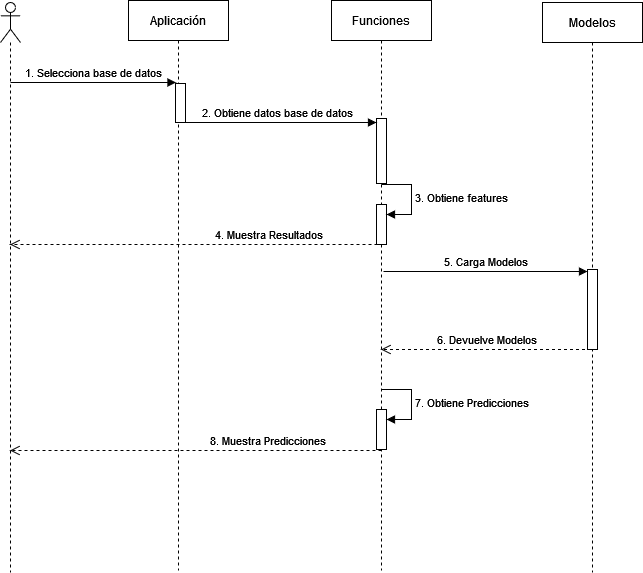
\includegraphics[width=0.9\textwidth]{img/secu.png}
 \caption{Diagrama de Secuencia}
 \label{f:secu}
\end{figure}

\section{Diseño arquitectónico}
En el diseño arquitectónico que compone la aplicación se pueden identificar tres elementos principales:
\begin{itemize}
    \item \textbf{Aplicación:} es un \emph{notebook} formado por tan solo tres celdas que permite al usuario poder seleccionar la base de datos a la que conectarse y posteriormente elegir la bobina o bobinas sobre las que se desea realizar predicciones.
    \item \textbf{Funciones:} es un fichero de \emph{Python} que contiene las diversas funciones que permiten el intercambio de flujo entre la aplicación y las diferentes funciones. Además, es capaz de calcular las diferentes \emph{features} y mostrar las predicciones de las bobinas. Finalmente, permite también generar CSV sobre las bobinas y llevar un registro sobre las diferentes predicciones en un fichero de texto.
    \item \textbf{Modelos:} son los encargados de efectuar las predicciones sobre los datos que genera la parte de funciones.
\end{itemize}

